\setmodule{9}

%BEGIN_FOLD % ====>>_____ Занятие 1 _____<<====
\begin{class}[number=1]
		%G111M6L1 L2
		%\item Площадь грани прямоугольного параллелепипеда равна \( 15 \). Ребро, перпендикулярное этой грани, равно \(3\). Найдите объем параллелепипеда.
		%\item Три ребра прямоугольного параллелепипеда, выходящие из одной вершины, равны \(4, 6, 9\). Найдите ребро равновеликого ему куба.
		%\item Два ребра прямоугольного параллелепипеда, выходящие из одной вершины, равны \(3\) и \(4\). Площадь поверхности этого параллелепипеда равна \(94\). Найдите третье ребро, выходящее из той же вершины.
		%\item Объем прямоугольного параллелепипеда равен \(24\). Одно из его ребер равно \(3\). Найдите площадь грани параллелепипеда, перпендикулярной этому ребру.
		%\item Прямоугольный параллелепипед описан около сферы радиуса \(1\). Найдите его площадь поверхности.
		%\item Диагональ куба равна \( 2\sqrt{3} \). Найдите объем куба и площадь его поверхности.
		%\item Объем первого куба в \( 8 \) раз больше объема второго куба. Во сколько раз площадь поверхности первого куба больше площади поверхности второго куба?
		%\item Найдите площадь боковой поверхности правильной шестиугольной призмы, сторона основания которой равна \( 5 \), а высота  --- \( 10 \).
		%\item Дан куб \( ABCDA_1B_1C_1D_1 \). Площадь четырехугольника \( ABC_1D_1 \) равна \( 4\sqrt{2} \). Найдите площадь поверхности куба.
		%\item 
		%\begin{minipage}[t]{\bodywidth}
		%	В правильной треугольной пирамиде \(SABC\) с вершиной \(S\) биссектрисы треугольника \(ABC\) пересекаются в точке \(O\). Площадь треугольника \(ABC\) равна \(2\); объем пирамиды равен \(6\). Найдите длину отрезка \(OS\).
		%\end{minipage}
		%\hspace{0.02\linewidth}
		%\begin{minipage}[t]{\picwidth}
		%	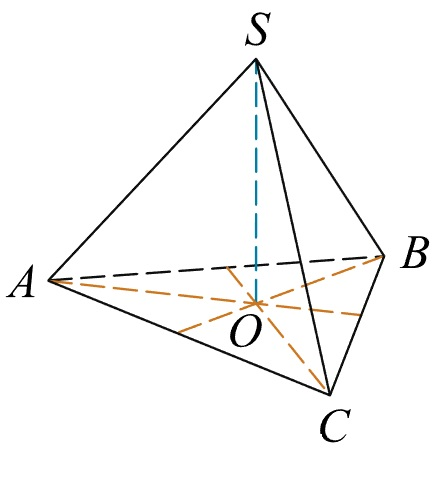
\includegraphics[align=t, width=\linewidth]{\picpath/G111M6L1-1}
		%\end{minipage}
		%\item В правильной четырехугольной пирамиде \(SABCD\) точка \(O\) --- центр основания, \(S\) --- вершина, \(SO=15, BD=16\). Найдите боковое ребро \(SA\).
		%
		%\item 
		%\begin{minipage}[t]{\bodywidth}
		%	В правильной треугольной пирамиде \(SABC\) точка \(M\) --- середина ребра \(AB\), \(S\) --- вершина. Известно, что \(BC = 3\), а площадь боковой поверхности пирамиды равна \(45\). Найдите длину отрезка \(SM\).
		%\end{minipage}
		%\hspace{0.02\linewidth}
		%\begin{minipage}[t]{\picwidth}
		%	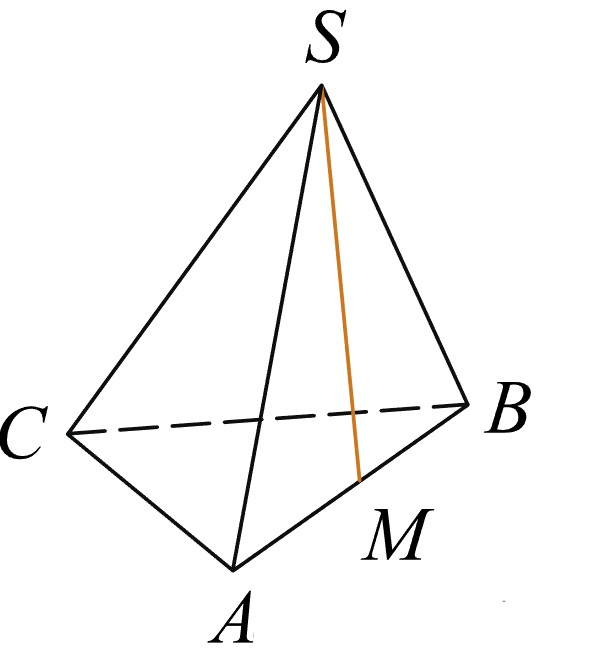
\includegraphics[align=t, width=\linewidth]{\picpath/G111M6L1-2}
		%\end{minipage}
		%\item Объем параллелепипеда \(ABCDA_1B_1C_1D_1\) равен \(9\). Найдите объем треугольной пирамиды \(ABCA_1\).
		%\item Во сколько раз увеличится объем правильного тетраэдра, если все его ребра увеличить в два раза?
		%\item В треугольнике \(ABC\) \(AB = 10, AC = BC\), высота \(AH = 8\). Найдите \(\cos{BAC}\).
		%\item В треугольнике со сторонами \(9\) и \(6\) проведены высоты к этим сторонам. Высота, проведённая к первой из этих сторон, равна \(4\). Чему равна высота, проведённая ко второй стороне?
		%\item Площадь параллелограмма \(ABCD\) равна \(24\). Точка \(M\) --- середина стороны \(BC\). Найдите площадь трапеции \(AMCD\).
		%\item 
		%\begin{minipage}[t]{\bodywidth}
		%	На рисунке изображен многогранник, все двугранные углы многогранника прямые. Найдите квадрат расстояния между вершинами \(B_2\) и \(D_3\) .
		%\end{minipage}
		%\hspace{0.02\linewidth}
		%\begin{minipage}[t]{\picwidth}
		%	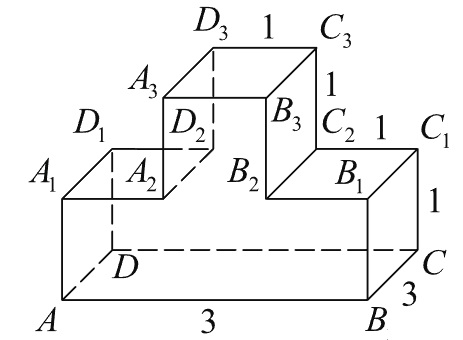
\includegraphics[align=t, width=\linewidth]{\picpath/G101M5L6-2}
		%\end{minipage}
		%\item 
		%\begin{minipage}[t]{\bodywidth}
		%	На рисунке изображен многогранник, все двугранные углы многогранника прямые. Найдите его объём и площадь поверхности.
		%\end{minipage}
		%\hspace{0.02\linewidth}
		%\begin{minipage}[t]{\picwidth}
		%	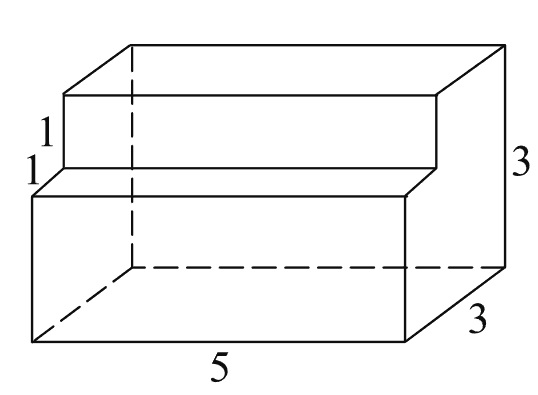
\includegraphics[align=t, width=\linewidth]{\picpath/G101M5L7-2}
		%\end{minipage}
		\begin{definit}
			Угол между пересекающимися плоскостями --- это наименьший из двугранных углов, образованных этими плоскостями.
			Угол между плоскостями равен углу между прямыми, соответственно перпендикулярными эти плоскостям.
		\end{definit}
		\begin{definit}
			Если одну из плоскостей заменить на параллельную, то полученный угол будет равен данному.
		\end{definit}
	\begin{listofex}
		%С27 1-3
		\item Дан куб \(ABCDA_1B_1C_1D_1\). Найдите угол между плоскостями:
		\begin{tasks}(2)
			\task \( BCC_1 \) и \( ABC_1 \);
			\task \( ABC \) и \( CB_1D_1 \);
			\task \( BA_1C_1 \) и \( AB_1D_1 \);
			\task \( ABC_1 \) и \( BCD_1 \).
		\end{tasks}
		\item Дан правильный тетраэдр \(ABCD\). Точки \(K\) и \(M\) --- середины рёбер \(BD\) и \(CD\) соответственно. Найдите углы между плоскостями:
		\begin{tasks}(3)
			\task \( AKC \) и \( ABD \);
			\task \( AMB \) и \( ABC \);
			\task \( AKM \) и \( ABC \).
		\end{tasks}
		\item Дана правильная четырёхугольная пирамида \(SABCD\) с вершиной \(S\). Все рёбра пирамиды равны, \(E\) --- середина бокового ребра \(SC\). Найдите углы между плоскостями:
		\begin{tasks}(3)
			\task \( SAD \) и \( SBC \);
			\task \( ABC \) и \( SCD \);
			\task \( ABC \) и \( BDE \).
			%\task \( BSC \) и \( DSC \).
			%\task \( ABE \) и \( ABC \).
		\end{tasks}
	\end{listofex}
	\begin{definit}
		Углом между прямой и плоскостью называется угол между прямой и её ортогональной проекцией на плоскость.
	\end{definit}
	\begin{listofex}[resume]
		%c45 1-2
		\item Дан куб \(ABCDA_1B_1C_1D_1\). Найдите углы:
		\begin{tasks}(1)
			\task между прямой \( AC_1 \) и плоскостью \(BDD_1 \);
			\task между прямой \(  AB\) и плоскостью \( CB_1D_1\);
			\task между прямой \( DD_1 \) и плоскостью \( ACB_1\);
			\task между прямой \( AC \) и плоскостью \( BCD_1\);
		\end{tasks}
		\item Дан правильный тетраэдр \(ABCD\). Точки \(K, M\) и \(N\) --- середины рёбер \(BD, AB\) и \(AC\) соответственно. Найдите углы:
		\begin{tasks}(1)
			\task между прямой \( CD \) и плоскостью \(ABD \);
			\task между прямой \(  DM\) и плоскостью \( ADC \);
			\task между прямой \( KN \) и плоскостью \( ADC\);
			\task между прямой \( BD \) и плоскостью \( KMN\);
		\end{tasks}
	\end{listofex}
\end{class}
%END_FOLD

%BEGIN_FOLD % ====>>_____ Занятие 2 _____<<====
\begin{class}[number=2]
	\begin{listofex}
		%c45 1-2
		\item Дан куб \(ABCDA_1B_1C_1D_1\). Найдите углы:
		\begin{tasks}(1)
			\task между прямой \( AC_1 \) и плоскостью \(BDD_1 \);
			\task между прямой \(  AB\) и плоскостью \( CB_1D_1\);
			\task между прямой \( DD_1 \) и плоскостью \( ACB_1\);
			\task между прямой \( AC \) и плоскостью \( BCD_1\);
		\end{tasks}
		\item Дан правильный тетраэдр \(ABCD\). Точки \(K, M\) и \(N\) --- середины рёбер \(BD, AB\) и \(AC\) соответственно. Найдите углы:
		\begin{tasks}(1)
			\task между прямой \( CD \) и плоскостью \(ABD \);
			\task между прямой \(  DM\) и плоскостью \( ADC \);
			\task между прямой \( KN \) и плоскостью \( ADC\);
			\task между прямой \( BD \) и плоскостью \( KMN\);
		\end{tasks}
		\item Дан правильный тетраэдр \(ABCD\). Точки \(K\) и \(M\) --- середины рёбер \(BD\) и \(CD\) соответственно. Найдите углы между плоскостями:
		\begin{tasks}(3)
			\task \( AKC \) и \( ABD \);
			\task \( AMB \) и \( ABC \);
			\task \( AKM \) и \( ABC \).
		\end{tasks}
		\item Дана правильная четырёхугольная пирамида \(SABCD\) с вершиной \(S\). Все рёбра пирамиды равны, \(E\) --- середина бокового ребра \(SC\). Найдите углы между плоскостями:
		\begin{tasks}(3)
			\task \( SAD \) и \( SBC \);
			\task \( ABC \) и \( SCD \);
			\task \( ABC \) и \( BDE \).
			%\task \( BSC \) и \( DSC \).
			%\task \( ABE \) и \( ABC \).
		\end{tasks}
	\end{listofex}
\end{class}
%END_FOLD

%BEGIN_FOLD % ====>>_ Домашняя работа 1 _<<====
\begin{homework}[number=1]
	\begin{listofex}
		\item Домашняя работа 1
	\end{listofex}
\end{homework}
%END_FOLD

%BEGIN_FOLD % ====>>_____ Занятие 3 _____<<====
\begin{class}[number=3]
	\begin{listofex}
		\item Занятие 3 
	\end{listofex}
\end{class}
%END_FOLD

%BEGIN_FOLD % ====>>_____ Занятие 4 _____<<====
\begin{class}[number=4]
	\begin{listofex}
		\item Занятие 4
	\end{listofex}
\end{class}
%END_FOLD

%BEGIN_FOLD % ====>>_ Домашняя работа 2 _<<====
\begin{homework}[number=2]
	\begin{listofex}
		\item Домашняя работа 2
	\end{listofex}
\end{homework}
%END_FOLD

%BEGIN_FOLD % ====>>_____ Занятие 5 _____<<====
\begin{class}[number=5]
	\begin{listofex}
		\item Занятие 5
	\end{listofex}
\end{class}
%END_FOLD

%BEGIN_FOLD % ====>>_____ Занятие 6 _____<<====
\begin{class}[number=6]
	\begin{listofex}
		\item Занятие 6
	\end{listofex}
\end{class}
%END_FOLD

%BEGIN_FOLD % ====>>_ Домашняя работа 3 _<<====
\begin{homework}[number=3]
	\begin{listofex}
		\item Домашняя работа 3
	\end{listofex}
\end{homework}
%END_FOLD

%BEGIN_FOLD % ====>>_____ Занятие 7 _____<<====
\begin{class}[number=7]
	\title{Подготовка к проверочной}
	\begin{listofex}
		\item Занятие 7
	\end{listofex}
\end{class}
%END_FOLD

%BEGIN_FOLD % ====>>_ Проверочная работа _<<====
\begin{exam}
	\begin{listofex}
		\item Проверочная
	\end{listofex}
\end{exam}
%END_FOLD